\section{EXECUTION-FEEDBACK CLOSED-LOOP COORDINATION}\label{sec:ecc}

This section addresses the second question of Section~\ref{sec:mission}. The hierarchy of Section~\ref{sec:framework} separates long-horizon decisions from constrained execution, but it also separates what the two layers know, and a decision layer trained only on realized transitions faces three mismatches with its executor. 1)~\textit{Information:} the execution layer can tell whether an intent will be converted into an entry, whereas the policy must infer this from sparse terminal outcomes; the state-level channel of Section~\ref{sec:feedback} passes this knowledge to the critics. 2)~\textit{Time scale:} decisions are taken once per stage, while passes recur once per spin period; the mode prediction of the execution layer spans $\Tp$, which covers a pass, and the action-level channel of Section~\ref{sec:screening} uses it at every decision. 3)~\textit{Consequence:} when $\eta<1$, neighboring intents can lead to capture and timeout, respectively, so that the value exhibits cliffs located by executor rules; the action-level channel corrects a proposal that would miss the last pass. Because the correction changes the transitions that the policy experiences, learning must take place under the same correction, which is the subject of Section~\ref{sec:consistent}. Learning itself remains off-policy temporal-difference learning on real transitions; the execution layer generates no value labels.

\begin{figure*}[t]
\centering
\begin{minipage}[b]{0.27\textwidth}\centering
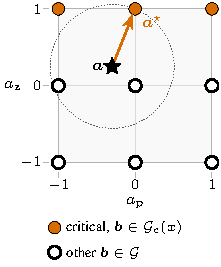
\includegraphics{figures/fig_screen_a.pdf}\\[2pt]{\footnotesize (a)}
\end{minipage}\hfill
\begin{minipage}[b]{0.35\textwidth}\centering
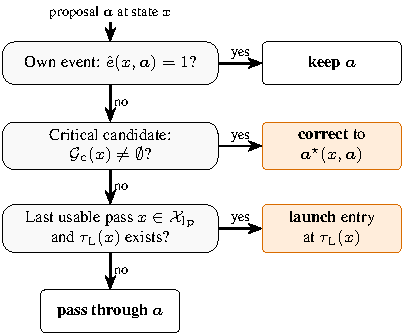
\includegraphics{figures/fig_screen_b.pdf}\\[2pt]{\footnotesize (b)}
\end{minipage}\hfill
\begin{minipage}[b]{0.36\textwidth}\centering
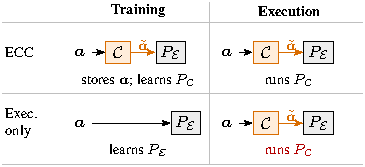
\includegraphics{figures/fig_screen_c.pdf}\\[2pt]{\footnotesize (c)}
\end{minipage}
\caption{Execution-opportunity screening. (a) Correction on the action box: the proposal $\ba$ triggers no mode event and is replaced by the nearest admissible candidate $\atil$; the dotted circle is the distance level set through $\atil$. (b) Critical-window condition of \eqref{eq:admissible}: the event predicted at $t+\tauhat$ is critical because the next pass, one spin period later, falls after $\te$. (c) Kernels learned and executed: with screening in training and execution, the policy is learned and executed under $\PC$; with screening at execution only, it is learned under $\PE$ but executed under $\PC$.}
\label{fig:screen}
\end{figure*}

\subsection{Macro-Step Decision Process}\label{sec:mdp}

Decisions are taken at the instants $t_{k}$ at which a macro step begins in mode $\modeS$ or $\modeH$, with the decision state $x_{k}$ of Definition~\ref{def:interface}. The policy reads the observation
\begin{equation}\label{eq:obs}
\begin{aligned}
\bo=\bigl[&\rho,\ (\bR_{\mathrm{s}}^{\T}\bv)^{\T},\ \psi,\ \dlat,\ \sin\varphi,\ \cos\varphi,\ \Omega,\\
&\Td-t,\ \iota,\ \Delta v,\ \Bmax-\Delta v,\ m_{\mathrm{b}},\ \beta,\ (\bR_{\mathrm{s}}^{\T}\bn)^{\T}\bigr]^{\T},
\end{aligned}
\end{equation}
where $\bR_{\mathrm{s}}=[\er,\epol,\eaz]$ resolves the relative velocity and the port direction in the basis of Section~\ref{sec:geometry}, $\psi=\psi(0)$ is the current port--line-of-sight angle, $\iota\in\{0,1\}$ is a mission indicator that identifies the cost weights, and $m_{\mathrm{b}}$ is the radial braking margin of Section~\ref{sec:entry}. The observation thus expresses the sweep-cone geometry directly, together with the remaining time and propellant; each entry is normalized by a fixed physical scale. The relative attitude is regulated by the execution layer and is not observed by the policy.

The intent $\ba_{k}\in\Aset$ is proposed by the policy and executed, after the correction of Section~\ref{sec:screening}, until the macro step ends. The reward of the macro step is
\begin{equation}\label{eq:reward}
r_{k}=\sum_{j\in\mathcal{J}_{k}}\bigl(-c_{\mathrm{t}}\Delta t-c_{\mathrm{f}}\Delta v_{j}\bigr)+r_{\mathrm{term}},
\end{equation}
where $\mathcal{J}_{k}$ collects the control periods of the macro step, $\Delta v_{j}$ is the velocity increment of period $j$, and $r_{\mathrm{term}}$ is $+100$ at capture, $-100$ at timeout ($t\ge\Td$), $-100$ at fuel exhaustion ($\Delta v\ge\Bmax$), $-150$ at an unsafe state ($X\notin\Sset$), and $0$ otherwise. Each of the four events terminates the process, which is indicated by $\chi_{k+1}=1$. For a captured task, the return $G=\sum_{k}r_{k}$ equals $100$ minus the cost of Problem~1, so that maximizing $\E[G]$ is the penalty form of \eqref{eq:problem}. A constant discount $\gamma$ is applied per decision. Training uses the potential-based shaped reward
\begin{equation}\label{eq:shaping}
\begin{aligned}
\rtil_{k}&=r_{k}+\gamma\Phi(x_{k+1})-\Phi(x_{k}),\\
\Phi(x)&=-\min\bigl\{\bar\ell_{\Phi},\ \norm{\brho-\brhom(t+\tau_{\Phi})}\bigr\},
\end{aligned}
\end{equation}
with $\Phi=0$ at termination, which attracts the chaser toward the mouth point predicted $\tau_{\Phi}$ ahead and leaves the optimal policies unchanged \cite{ng1999shaping}. All evaluations report the return $G$ of the unshaped reward \eqref{eq:reward}.

\subsection{State-Level Channel: Execution Feedback}\label{sec:feedback}

The execution feedback of Definition~\ref{def:interface} consists of three opportunity judgments and three execution-status quantities,
\begin{equation}\label{eq:zE}
\bz=\bigl[\taup,\ \min_{\tau\in\Tset}\hat\psi(\tau),\ \Td-t-\taup-T_{\mathrm{o}},\ d_{\rho},\ d_{v},\ i_{\modeH}\bigr]^{\T}.
\end{equation}
The first item is the time $\taup=\varphi/\Omega$ to the next pass, the second is the closest port alignment over the candidate arrival times of \eqref{eq:entry}, and the third is the deadline margin left after the pass once a fixed time $T_{\mathrm{o}}$ for the final phase is deducted; it differs from $\eta\Ts$ in \eqref{eq:eta} only by the constant $T_{\mathrm{o}}-\Tr$. The remaining items are the position and velocity deviations $d_{\rho}$ and $d_{v}$ of the previous stage from its plan and the indicator $i_{\modeH}\in\{0,1\}$ of the hold mode. The actor and the two critics are
\begin{equation}\label{eq:asym}
\pi_{\vect{\theta}}(\ba\,|\,\bo),\qquad Q_{\vect{\zeta}_{i}}(\bo,\bz,\ba),\quad i=1,2.
\end{equation}
For the same observation, $\bz$ distinguishes whether an opportunity actually exists and whether the previous intent was executed as planned, so that the critics can represent values closer to the realized consequences of execution. The feedback is used only by the critics during training; at execution, the policy acts on $\bo$ alone.

\subsection{Action-Level Channel: Execution-Opportunity Screening}\label{sec:screening}

The action-level channel rests on a question that the execution layer answers from its own rules: if an intent were held from now on, would the execution layer leave stage flight, and if so, when and at what propellant cost?

\begin{definition}[Mode prediction]\label{def:pred}
The mode prediction is the map $\Mpred:\Xset\times\Aset\to\{0,1\}\times[0,\Tp]\times\R_{\ge0}$, $(x,\bb)\mapsto(\ehat,\tauhat,\dvhat)$, where $\ehat=1$ if and only if, under the prediction \eqref{eq:pred} and with the intent $\bb$ held, the rules of Section~\ref{sec:framework} produce the terminal descent or a feasible entry within $\Tp$, $\tauhat$ is the time of this event or the time at which the prediction stops, and $\dvhat$ is the planned velocity increment up to the event, including the entry plan.
\end{definition}

The prediction rolls out the stage goals \eqref{eq:goal} and the stage plans of Problem~2 for up to $\Tp/h$ stages, treating a rejected stage as a hold, and applies the descent condition of Table~\ref{tab:modes} and the entry condition \eqref{eq:entry} every $\Tm$ along the planned path. It stops at the first event, at $\Tp$, at the deadline, or when the planned propellant exhausts the budget. It uses no data from past tasks, evaluates no rewards or values, and runs on separate planner instances, so that the executed trajectory is the same whether or not a prediction is made. A predicted event is a mode switch in the model of the execution layer, not a capture.

Let $\Gset\subset\Aset$ be a finite set of candidate intents; this article uses the uniform grid $\Gset=\{-1,0,1\}^{2}$, which covers the action box with its center, edges, and vertices. The admissible candidate set is
\begin{equation}\label{eq:admissible}
\begin{aligned}
\Ga(x)=\bigl\{\bb\in\Gset:\ & \ehat(x,\bb)=1,\ \ t+\tauhat(x,\bb)+\Ts>\te,\\
& \Delta v+\dvhat(x,\bb)\le\Bmax\bigr\}.
\end{aligned}
\end{equation}
The three conditions require that the candidate trigger an entry or a descent, that the event belong to a critical window, and that the candidate be affordable. The second condition is the predicted counterpart of $\eta<1$ in \eqref{eq:eta}: with the predicted event in place of the pass center, it states that missing the event leaves no further pass before $\te$ (Fig.~\ref{fig:screen}(b)). The correction map is
\begin{equation}\label{eq:correction}
\Cmap(x,\ba)=
\begin{cases}
\ba, & \text{if }\ehat(x,\ba)=1\text{ or }\Ga(x)=\emptyset,\\
\ba^{\star}(x,\ba), & \text{otherwise},
\end{cases}
\end{equation}
with $\ba^{\star}(x,\ba)\in\argmin_{\bb\in\Ga(x)}\norm{\bb-\ba}$,
where ties in the minimization are broken by the smaller $\tauhat(x,\bb)$ and then by a fixed order of $\Gset$. The executed intent is $\atil=\Cmap(x,\ba)$ (Fig.~\ref{fig:screen}(a)); the correction applies to the current macro step only.

\begin{property}\label{prop:correction}
For every $x\in\Xset$ and $\ba\in\Aset$: (i)~$\Cmap(x,\ba)=\ba$ if $\ehat(x,\ba)=1$ or $\Ga(x)=\emptyset$; (ii)~otherwise $\Cmap(x,\ba)\in\Ga(x)$ and $\norm{\Cmap(x,\ba)-\ba}=\min_{\bb\in\Ga(x)}\norm{\bb-\ba}$; (iii)~$\Cmap$ is single valued and idempotent, $\Cmap(x,\Cmap(x,\ba))=\Cmap(x,\ba)$.
\end{property}

Items (i) and (ii) restate \eqref{eq:correction}; the minimizer exists because $\Ga(x)$ is finite. The tie-breaking rule and the deterministic prediction make $\Cmap$ single valued, and a corrected intent lies in $\Ga(x)$, so it triggers an event and is left unchanged by a second application. Screening therefore acts only when the proposal would miss a critical window that a candidate can use, and then changes the intent as little as the candidate set allows. Each decision requires $|\Gset|+1$ mode predictions, each with at most $\Tp/h$ stage plans and $|\Tset|\Tp/\Tm$ entry plans. Screening is a test on the model of the execution layer; it guarantees neither safety nor capture.


\subsection{Training--Execution Consistent Learning}\label{sec:consistent}

Screening modifies the transitions of the closed loop. Applied only at execution, it acts as a postprocessing filter that is invisible during learning, and the policy is optimized for a system other than the one it controls \cite{reiter2026arc}. ECC applies the same map $\Cmap$ in training and execution (Fig.~\ref{fig:screen}(c)). The screened kernel is
\begin{equation}\label{eq:PC}
\PC(x',r\,|\,x,\ba)=\PE\bigl(x',r\,|\,x,\Cmap(x,\ba)\bigr),
\end{equation}
and the replay buffer stores the proposed intent $\ba$, not $\atil$, together with the reward and the successor obtained by executing $\atil$. The critics thus learn what happens when the policy proposes $\ba$.

\begin{proposition}[Screened decision process]\label{prop:screen}
Let transitions be collected by proposing $\ba_{k}\sim\pi(\cdot\,|\,\bo_{k})$, executing $\Cmap(x_{k},\ba_{k})$, and storing $(\bo_{k},\bz_{k},\ba_{k},\rtil_{k},\bo_{k+1},\bz_{k+1},\chi_{k+1})$.
\begin{enumerate}
\item The stored transitions are samples of the decision process $(\Xset,\Aset,\PC,\rtil,\gamma)$, and the temporal-difference target formed from a stored transition is a sample of its Bellman operator
\begin{equation}\label{eq:bellman}
(\mathcal{B}^{\pi}Q)(x,\ba)=\E_{\PC}\Bigl[\rtil+\gamma(1-\chi')\,\E_{\ba'\sim\pi}Q(x',\ba')\Bigr].
\end{equation}
\item If $\Cmap(x,\ba_{1})=\Cmap(x,\ba_{2})$, then $\PC(\cdot\,|\,x,\ba_{1})=\PC(\cdot\,|\,x,\ba_{2})$ and $Q^{\pi}_{\mathcal{C}}(x,\ba_{1})=Q^{\pi}_{\mathcal{C}}(x,\ba_{2})$ for every policy $\pi$.
\item Let $\Pi$ be a class of observation-feedback policies and $V_{\mathcal{C}}(\pi)$ and $V_{\mathcal{E}}(\pi)$ the expected discounted returns of $\pi$ under $\PC$ and $\PE$. The system executed with screening attains $V_{\mathcal{C}}(\pi)$ for every $\pi\in\Pi$; hence any $\pi_{\mathcal{C}}\in\argmax_{\Pi}V_{\mathcal{C}}$ performs on it at least as well as every policy of $\Pi$, including any $\pi_{\mathcal{E}}\in\argmax_{\Pi}V_{\mathcal{E}}$.
\end{enumerate}
\end{proposition}

\textit{Proof:} (i)~By Definition~\ref{def:interface}, $x_{k}$ determines the evolution over a macro step once the executed intent is fixed. The mode prediction runs on separate planner instances and leaves $x_{k}$ unchanged, and $\Cmap$ is a deterministic function of $(x_{k},\ba_{k})$ by Property~\ref{prop:correction}. Hence, conditioned on $(x_{k},\ba_{k})$, the pair $(x_{k+1},r_{k})$ is distributed according to $\PE(\cdot\,|\,x_{k},\Cmap(x_{k},\ba_{k}))=\PC(\cdot\,|\,x_{k},\ba_{k})$, regardless of how $\ba_{k}$ was sampled. The shaped reward is a function of $(x_{k},r_{k},x_{k+1})$ and $\chi_{k+1}$ a function of $x_{k+1}$, so the stored transitions are samples of this decision process, and the target $\rtil_{k}+\gamma(1-\chi_{k+1})\E_{\ba'\sim\pi}Q(x_{k+1},\ba')$ is a sample of \eqref{eq:bellman} at $(x_{k},\ba_{k})$. (ii)~By \eqref{eq:PC}, $\PC(\cdot\,|\,x,\ba)$ depends on $\ba$ only through $\Cmap(x,\ba)$, and so does the fixed point of \eqref{eq:bellman}. (iii)~At execution, a proposal $\ba\sim\pi(\cdot\,|\,\bo)$ is executed as $\Cmap(x,\ba)$, so the executed system follows $\PC$ and its return under $\pi$ is $V_{\mathcal{C}}(\pi)$; the inequality is the definition of a maximizer. Since the shaped and unshaped returns of any policy differ by $-\E[\Phi(x_{0})]$, the maximizers are the same for both rewards. \hfill$\square$

By Proposition~\ref{prop:screen}(ii), proposals mapped to the same candidate have the same value, so the policy need not learn to emit the corrected intent itself; policy and correction act as one decision rule. Proposition~\ref{prop:screen}(iii) states the consequence for the alternatives: a policy trained without screening and executed with it is in general not the best policy for the system it controls, and a policy trained with screening is matched to that system, so that removing screening at execution changes the system it was trained for. It compares optimal values under screening and does not compare a system with screening to one without it.

\begin{remark}\label{rem:related}
Asymmetric actor--critic methods train the critic on privileged simulator states \cite{pinto2018asymmetric}, shielding places a correction layer in the learning loop to enforce safety specifications \cite{alshiekh2018shielding}, postprocessing filters correct actions only at execution \cite{reiter2026arc}, and projection-based schemes learn from the corrected action or a mixture of corrected and original actions \cite{lu2025eaai}. The novelty of ECC lies in their combination for hierarchical RL--MPC. Both channels are supplied by the same execution-layer interface from the short-horizon prediction of the executor itself, rather than from simulator states or a separately synthesized monitor; the correction targets execution opportunities rather than safety, with a criterion derived from the time structure of the task; and the correction is placed so that the learning target is consistent with the executed system (Proposition~\ref{prop:screen}).
\end{remark}

The decision layer is trained with soft actor--critic (SAC) \cite{haarnoja2018sac} in the asymmetric form \eqref{eq:asym}. The policy is a Gaussian squashed by $\tanh$ onto $\Aset$, and the actor and the critics are fully connected networks with separate input layers. With target critics $Q_{\vect{\zeta}_{i}^{-}}$, the critic target and the losses are
\begin{align}
y&=\rtil+\gamma(1-\chi')\Bigl[\min_{i}Q_{\vect{\zeta}_{i}^{-}}(\bo',\bz',\ba')\nonumber\\
&\qquad\qquad-\alpha\log\pi_{\vect{\theta}}(\ba'\,|\,\bo')\Bigr],\label{eq:target}\\
\mathcal{L}(\vect{\zeta}_{i})&=\E\bigl[(Q_{\vect{\zeta}_{i}}(\bo,\bz,\ba)-y)^{2}\bigr],\nonumber\\
\mathcal{L}(\vect{\theta})&=\E\Bigl[\alpha\log\pi_{\vect{\theta}}(\ba_{\theta}\,|\,\bo)-\min_{i}Q_{\vect{\zeta}_{i}}(\bo,\bz,\ba_{\theta})\Bigr],\nonumber
\end{align}
where $\ba'\sim\pi_{\vect{\theta}}(\cdot\,|\,\bo')$, $\ba_{\theta}\sim\pi_{\vect{\theta}}(\cdot\,|\,\bo)$, $\alpha$ is a fixed temperature, and the expectations are taken over the replay buffer. Algorithm~\ref{alg:ecc} summarizes training and execution; at execution, the policy mean is used.

\begin{remark}\label{rem:scope}
Proposition~\ref{prop:screen} concerns the learning target on the decision state $x$; the actor on $\bo$ and the critics on $(\bo,\bz)$ are function approximations of it. No statement is made on the convergence of SAC, on safety, which is judged only on the dynamics \eqref{eq:kin}--\eqref{eq:fg}, or on whether screening improves over its absence; these effects are quantified in Section~\ref{sec:experiments}.
\end{remark}

\begin{algorithm}[t]
\caption{ECC Training and Execution}
\label{alg:ecc}
\small
\begin{algorithmic}[1]
\State Initialize $\pi_{\vect{\theta}}$, $Q_{\vect{\zeta}_{1}},Q_{\vect{\zeta}_{2}}$, targets, and buffer $\mathcal{D}$ \Comment{T}
\For{each decision in mode $\modeS$ or $\modeH$}
  \State Observe $\bo$ (and $\bz$ in training); propose $\ba\sim\pi_{\vect{\theta}}(\cdot\,|\,\bo)$ (mean at execution)
  \State Evaluate $\Mpred(x,\bb)$ for $\bb\in\Gset\cup\{\ba\}$; form $\Ga(x)$ by \eqref{eq:admissible}
  \State Set $\atil\gets\Cmap(x,\ba)$ by \eqref{eq:correction}
  \State Execute $\atil$ with RWG and MPC until the macro step ends
  \State Store $(\bo,\bz,\ba,\rtil,\bo',\bz',\chi')$ in $\mathcal{D}$ \Comment{T}
  \State Update the critics and the actor by \eqref{eq:target} \Comment{T}
\EndFor
\end{algorithmic}
\textit{Note:} Steps marked T are performed only in training; all other steps are shared by training and execution.
\end{algorithm}
